\documentclass[tikz, border=1mm]{standalone}
\begin{document}

\tikzset{every picture/.style={line width=0.75pt}} %set default line width to 0.75pt

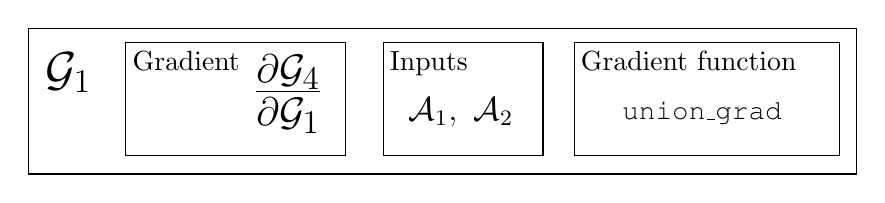
\begin{tikzpicture}[x=0.75pt,y=0.75pt,yscale=-1,xscale=1]
%uncomment if require: \path (0,300); %set diagram left start at 0, and has height of 300

%Shape: Rectangle [id:dp05199341754851439]
\draw   (113,131) -- (512,131) -- (512,201.25) -- (113,201.25) -- cycle ;
%Shape: Rectangle [id:dp39626246750052907]
\draw   (160,138) -- (266,138) -- (266,192.5) -- (160,192.5) -- cycle ;
%Shape: Rectangle [id:dp09229086143626253]
\draw   (284,138) -- (361,138) -- (361,192.5) -- (284,192.5) -- cycle ;
%Shape: Rectangle [id:dp2579586986982425]
\draw   (376,138) -- (504,138) -- (504,192.5) -- (376,192.5) -- cycle ;

% Text Node
\draw (120,141.4) node [anchor=north west][inner sep=0.75pt]    {\LARGE $\mathcal{G}_{1}$};
% Text Node
\draw (220,142.4) node [anchor=north west][inner sep=0.75pt]    {\huge $\frac{\partial \mathcal{G}_{4}}{\partial \mathcal{G}_{1}}$};
% Text Node
\draw (162,141) node [anchor=north west][inner sep=0.75pt]   [align=left] {Gradient};
% Text Node
\draw (286,141) node [anchor=north west][inner sep=0.75pt]   [align=left] {Inputs};
% Text Node
\draw (378,141) node [anchor=north west][inner sep=0.75pt]   [align=left] {Gradient function};
\draw (390,165) node [anchor=north west][inner sep=0.75pt]   [align=left] {{\fontfamily{pcr}\selectfont  \ union\_grad}};
% Text Node
\draw (295,163.4) node [anchor=north west][inner sep=0.75pt]    {\large $\mathcal{A}_{1} ,\ \mathcal{A}_{2}$};


\end{tikzpicture}
\end{document}
